%%%%%%%%%%%%%%%%%%%%%%%%%%%%%%%%%%%%%%%%%%%%%%%%%%%%%%%%%%%%%%%%%%%%
\section{Organization and Management}
\label{sec:fdsp-pd-org}
%\metainfo{\color{red}\bf  Content: Segreto/Warner}

The \dword{sp} \dword{pd} consortium benefits from the contributions of many institutions and facilities in Europe and North and South America.  Table~\ref{tab:sp-pds-institutes-i}
%and \ref{tab:sp-pds-institutes-ii} 
lists the member institutions. 
%To help guide the interactions of these many contributors, the consortium is divided into six working groups, each with two or three conveners, to direct its activities.  % The structure of the organization is detailed below.

%%%%%%%%%%%%%%%%%%%%%%%%%%%%%%%%%%%
%\subsection{Consortium Organization}
\label{sec:fdsp-pd-org-consortium}
%\fixme{Please remove org chart with names and add a list of institutions. Template provided. Anne 4/16}
%\fixme{Dave/Ettore: Table needs completing. The org chart needs to be commented out and the text changed to refer to the new table.}

\begin{longtable}
%[PDS Consortium Institutions]
{ll}
\caption{PD System Consortium Institutions}\\ \colhline
\rowcolor{dunetablecolor} Member Institute  &  Country       \\  \toprowrule
Federal University of ABC & Brazil \\ \colhline
State University of Feira de Santana & Brazil \\ \colhline
Federal University of Alfenas Po\c{c}os de Caldas & Brazil \\ \colhline
Centro Brasileiro de Pesquisas F\'isicas & Brazil \\ \colhline
Federal University of Goi\'as & Brazil \\ \colhline
Brazilian Synchotron Light Laboratory LNLS/CNPEM & Brazil \\ \colhline
University of Campinas & Brazil \\ \colhline
CTI Renato Archer & Brazil \\ \colhline
Federal Technological University of Paran\'a & Brazil \\ \colhline
Universidad del Atlantico & Colombia \\ \colhline
Universidad Sergia Ablada & Colombia \\ \colhline
University Antonio Nari\~{n}o & Colombia \\ \colhline
Institute of Physics CAS & Czech Republic \\ \colhline
Czech Technical University in Prague & Czech Republic \\ \colhline
Universidad Nacional de Assuncion & Paraguay \\ \colhline
Pontificia Universidad Catilica Per\'{u} & Per\'{u} \\ \colhline
Universidad Nacional de Ingineria & Per\'{u} \\ \colhline
University of Warwick & UK \\ \colhline
University of Sussex & UK \\ \colhline
University of Manchester & UK \\ \colhline
Edinburgh University & UK \\ \colhline
Argonne National Laboratory & UK \\\colhline
Brookhaven National Laboratory & UK \\ \colhline
California Institute of Technology & UK \\ \colhline
Colorado State University   &  USA  \\ \colhline
\dword{fnal}    &   USA    \\ \colhline
Duke University & USA \\ \colhline
Idaho State University & USA \\ \colhline
Indiana University & USA \\ \colhline
University of Iowa & USA \\ \colhline
Louisiana State University & USA \\ \colhline
Massachusetts Institute of Technology & USA \\ \colhline
University of Michigan & USA \\ \colhline
Northern Illinois University & USA \\ \colhline
South Dakota School of Mines and Technology & USA \\ \colhline
Syracuse University & USA \\ \colhline
University of Bologna and INFN & Italy \\ \colhline
University of Milano Bicocca and INFN & Italy \\ \colhline
University of Genova and INFN & Italy \\ \colhline
University of Catania and INFN & Italy \\ \colhline
Laboratori Nazionali del Sud & Italy \\ \colhline
University of Lecce and INFN & Italy \\ \colhline
INFN Milano & Italy \\ \colhline
INFN Padova & Italy \\  \colhline
\label{tab:sp-pds-institutes-i}
\end{longtable}

%\begin{comment}
%\begin{dunetable}
%[PDS Consortium Institutions - Part II]
%{ll}
%{tab:sp-pds-institutes-ii}
%{PDS Consortium Institutions - Part II}
%Member Institute         &  Country       \\  \colhline
%University of Genova and INFN & Italy \\ \colhline
%University of Catania and INFN & Italy \\ \colhline
%Laboratori Nazionali del Sud & Italy \\ \colhline
%University of Lecce and INFN & Italy \\ \colhline
%INFN Milano & Italy \\ \colhline
%INFN Padova & Italy \\ 
%\end{dunetable}
%\end{comment}

The \single \dword{pds} consortium follows the typical organizational structure of DUNE consortia:
\begin{itemize}
\item A Consortium Lead provides overall leadership for the effort, and attends meetings of the DUNE Executive and Technical Boards.
\item A Technical Lead provides technical support to the consortium lead, attends the Technical Board and other project meetings, oversees the project schedule and \dword{wbs}, and oversees the operation of the project working groups.  
%In the case of the \dword{pds}, the technical lead is supported by a deputy technical lead.
\end{itemize}

%\begin{dunefigure}[PDS consortium organization chart]{fig:pds-org-chart}
%{\dword{pds} consortium organization chart.}

%	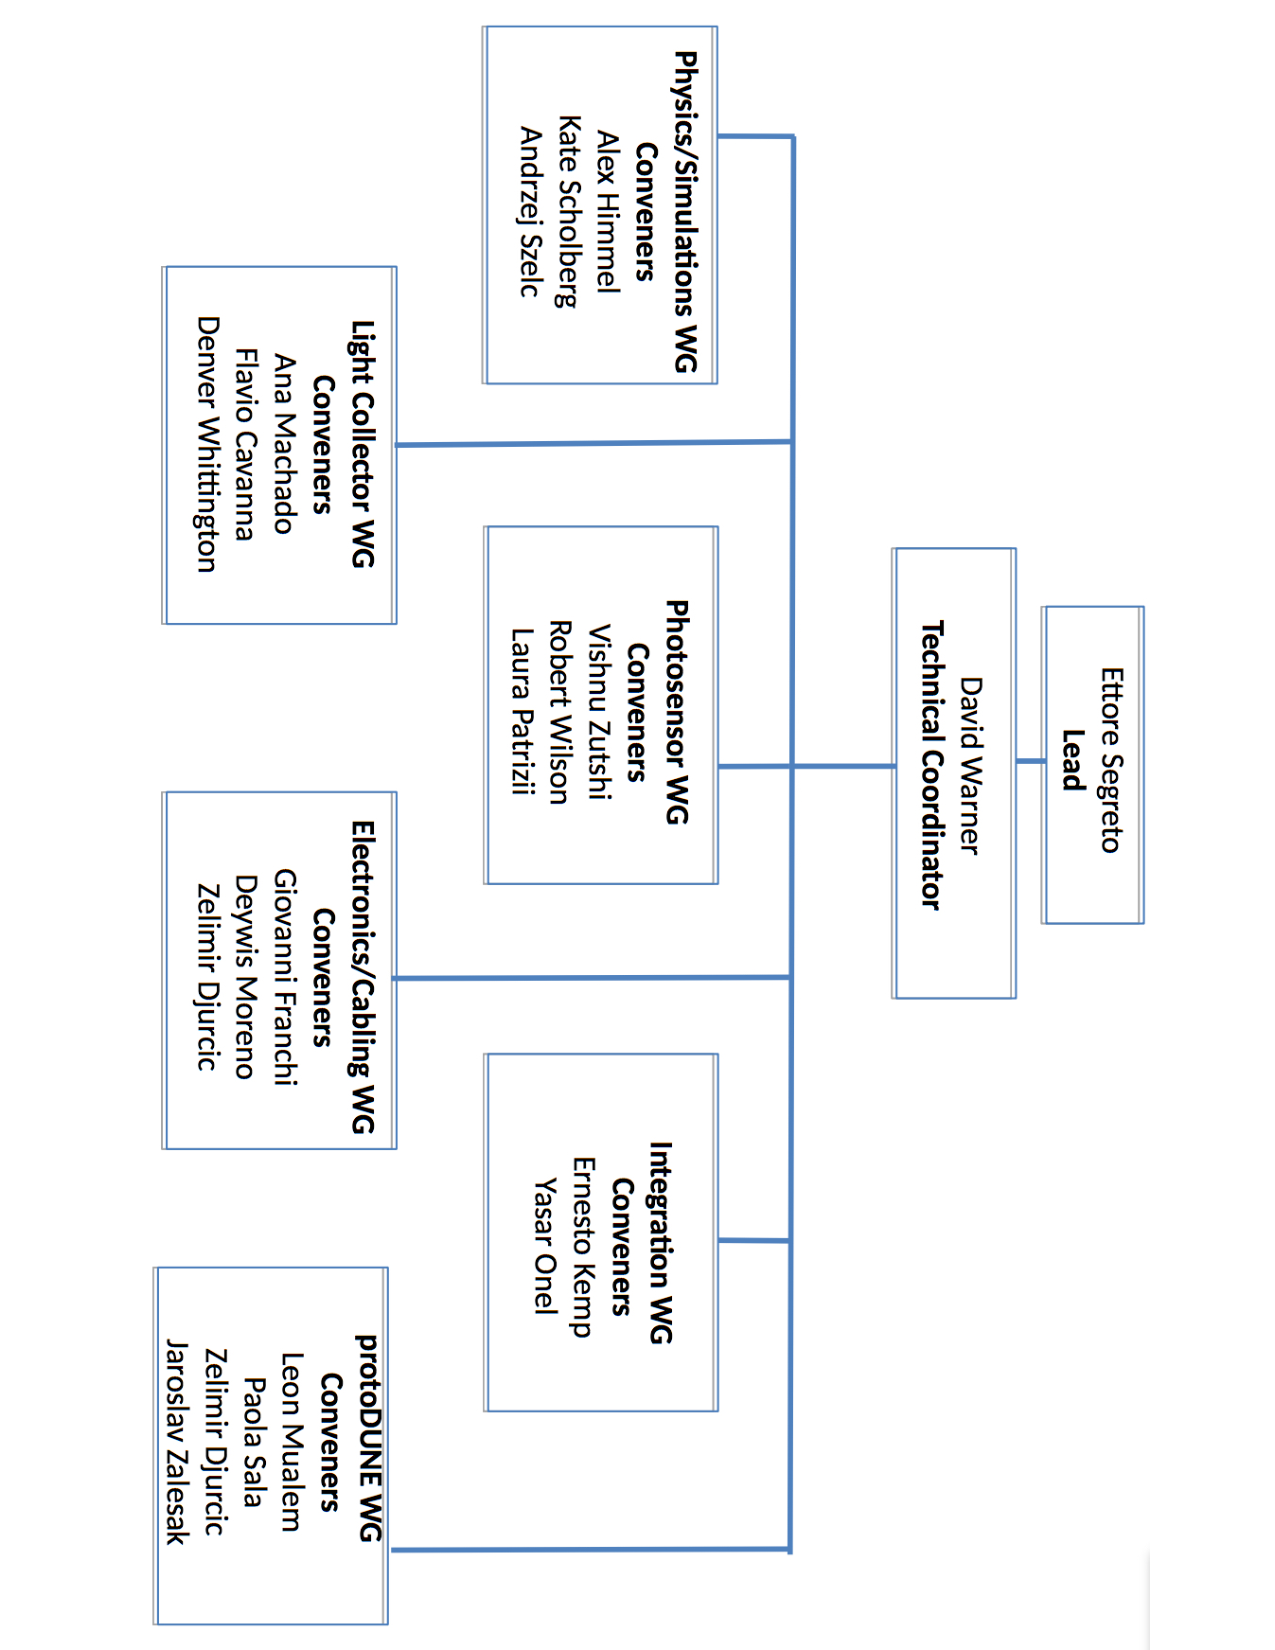
\includegraphics[angle=90,height=12cm]{pds-consortium-org-chart}
	
%\end{dunefigure} 

Below the leadership, the consortium is divided up into six working groups, each led by two or three working group conveners (see Table~\ref{tbl:pds-wgs}).  Each working group is charged with one primary area of responsibility within the consortium, and the conveners report directly to the Technical Lead regarding those responsibilities.

\begin{dunetable}[\dshort{pd} Working Groups]
{ll}
{tbl:pds-wgs}
{PD working groups and responsibilities}
Working Group			 & Responsibilities\\ \toprowrule
Light Collector WG & Mechanical design, materials selection for PD modules\\ \colhline
Photosensors WG & Selection, validation, procuring of photosensors, cold active ganging\\ \colhline
Readout electronics WG & Warm electronics, cable harness, DAQ interface\\ \colhline
Integration and Installation WG & Internal (inter-WG) and external (inter-consortia) interfaces\\ \colhline
Physics and Simulation WG & Physics and simulations studies to determine \dword{pd} specifications\\ \colhline
ProtoDUNE Analysis WG & Validation of PD system in \dshort{pdsp} and \dshort{pdsp2}\\
\end{dunetable}

The working group conveners are appointed by the \dword{pds} Consortium Lead and Technical Lead; the structure may evolve as the consortium matures and additional needs are identified. 


\subsection{High-Level Schedule}
\label{sec:fdsp-pd-org-cs}

Table \ref{tab:Xsched} lists key milestones in the design, validation construction and installation of the single-phase photon detector system.  These milestones include external milestones indicating linkages to the main DUNE schedule (highlighted in color in the table), as well as internal milestones such as design validation and technical reviews.

In general the flow of the schedule commences with a 60\% design review based module performance testing at ICEBERG and at \dword{unicamp}, and integration testing at Ash River.  Additional similar design validation follows, leading to a final design review (FDR).  Following the FDR, 30 modules and required electronics, cabling and \dword{pd} monitoring system components for \dword{pdsp2} will be built, installed and validated during a second ProtoDUNE run at \dword{cern}.  Once the data from this test have undergone initial analysis, production readiness reviews will be conducted and module fabrication will begin.

Some parts of the \dword{pds} system, such as the support rails and electrical connectors required in mid-2020 for \dword{apa} assembly, and photosensors and filter plates which have a long procurement cycle, will require an abbreviated design review process as detailed in the narrative earlier in this document and shown in the milestone table.

%\forlbnc{LBNC:  This section is a placeholder.  Milestones of \dword{pd} system development and fabrication are shown in order, however the integrated project schedule is still being developed and no dates are shown at this time.  The correct schedule milestone dates will be inserted into the final revision to be presented in July.}


%\fixme{This is a standard table template for the TDR schedules.  It contains overall FD dates from Eric James as of March 2019 (orange) that are held in macros in the common/defs.tex file so that the TDR team can change them if needed. Please do not edit these lines! Please add your milestone dates to fit in with the overall FD schedule. And fix table captions and label, please. (Anne)}


\begin{longtable}
%{11}
%[PDS Consortium Schedule]
{p{0.75\textwidth}p{0.25\textwidth}}
%{PDS Consortium Schedule}   
\caption{PD System Consortium schedule}\\ \colhline
\rowcolor{dunetablecolor}Milestone & Date   \\ \toprowrule
60 percent design validation testing complete & November 2019    \\ \colhline
60 percent design review & December 2019    \\ \colhline
Final design review for PD rails, cables, connectors & February 2020\\ \colhline
\dword{prr} for PD rails, cables. connectors & April 2020\\ \colhline
Fabrication of PD rails, cables, connectors begins & April 2020\\ \colhline
Final design validation testing complete & April 2020    \\ \colhline
Down selection to two photosensor candidates & May 2020\\ \colhline
Final design review for remaining PD components & May 2020\\ \colhline
Start of module 0 component production for \dword{pdsp2} & March 2021\\ \colhline
End of module 0 component production for \dword{pdsp2} & June 2021\\ \colhline
\rowcolor{dunepeach} Start of \dword{pdsp2} installation& \startpduneiispinstall      \\ \colhline
\dword{prr} for photosensors & July 2021\\ \colhline
Begin procurement of production photosensors  & July 2021\\ \colhline
End of module 0 installation for \dword{pdsp2} & August 2021\\ \colhline
Begin procurement of filter plates  & October 2021\\ \colhline
\dword{pdsp2} initial results available & December 2021\\ \colhline
\dword{prr} for remaining photon detector components & January 2022\\ \colhline
Begin fabrication/procurement of remaining module components & January 2022\\ \colhline
Begin assembly of PD monitoring system  & January 2022\\ \colhline
\rowcolor{dunepeach} Start of \dword{pdsp2} installation & \startpduneiidpinstall      \\ \colhline
Begin assembly of front-end electronics modules  & March 2022\\ \colhline
\rowcolor{dunepeach}\dshort{sdwf} available& \sdlwavailable      \\ \colhline
Begin assembly of X-ARAPUCA modules  & July 2022\\ \colhline
\rowcolor{dunepeach}Beneficial occupancy of cavern 1 and \dword{cuc}& \cucbenocc      \\ \colhline
Initial batch (80 PD modules) assembled  & March 2023\\ \colhline
\rowcolor{dunepeach} \dword{cuc} counting room accessible& \accesscuccountrm      \\ \colhline
Initial batch (80 PD modules) arrive at US PD Reception Facility  & June 2023\\ \colhline
Second batch (160 PD modules) assembled  & July 2023\\ \colhline
Initial batch (80 PD modules) arrive at \dshort{sdwf}  & September 2023\\ \colhline
Second batch (160 PD modules) arrive at US PD Reception Facility  & October 2023\\ \colhline
%(\#1 TPC) First 560 modules fabricated   & October 2023\\ \colhline
\dword{pd} monitoring system at \dshort{sdwf}   & October 2023\\ \colhline
Third batch (320 PD modules) assembled  & November 2023\\ \colhline
Second batch (160 PD modules) arrive at \dshort{sdwf}  & December 2023\\ \colhline
\rowcolor{dunepeach}Top of \dword{detmodule} \#1 cryostat accessible& \accesstopfirstcryo      \\ \colhline
Third batch (320 PD modules) arrive at US PD Reception Facility  & January 2024\\ \colhline
%(\#1 TPC) First 560 modules at \dshort{sdwf}   & April 2024\\ \colhline
%(\#1 TPC) 
Front end electronics modules at \dshort{sdwf}   & February 2024\\ \colhline
Fourth batch (320 PD modules) assembled  & February 2024\\ \colhline
Third batch (320 PD modules) arrive at \dshort{sdwf}  & April 2024\\ \colhline
Fourth batch (320 PD modules) arrive at US PD Reception Facility  & May 2024 \\ \colhline
Fifth batch (320 PD modules) assembled  & June 2024\\ \colhline
\rowcolor{dunepeach}Start of \dword{detmodule} \#1 TPC installation& \startfirsttpcinstall      \\ \colhline
Fourth batch (320 PD modules) arrive at \dshort{sdwf}  & August 2024\\ \colhline
Fifth batch (320 PD modules) arrive at US PD Reception Facility  & September 2024 \\ \colhline
Final batch (300 PD modules) assembled  & December 2024\\ \colhline
Fifth batch (320 PD modules) arrive at \dshort{sdwf}  & December 2024\\ \colhline
Final batch (300 PD modules) arrive at US PD Reception Facility  & February 2025 \\ \colhline
Final batch (300 PD modules) arrive at \dshort{sdwf}  & April 2025\\ \colhline
%(\#1 TPC) Final PD modules at \dshort{sdwf}   & April 2025\\ \colhline
\rowcolor{dunepeach}End of \dword{detmodule} \#1 TPC installation& \firsttpcinstallend      \\ \colhline
\rowcolor{dunepeach}Top of \dword{detmodule} \#2 accessible& \accesstopsecondcryo      \\ \colhline
%(\#2 TPC) \dword{pd} light collector modules at Logistics Warehouse   &    \\ \colhline
%(\#2 TPC) Remaining 1000 modules at Logistics Warehouse   &    \\ \colhline
%(\#2 TPC) Front end electronics modules at Logistics Warehouse   &    \\ \colhline
 \rowcolor{dunepeach}Start of \dword{detmodule} \#2 TPC installation& \startsecondtpcinstall      \\ \colhline
\rowcolor{dunepeach}End of \dword{detmodule} \#2 TPC installation& \secondtpcinstallend      \\ 
\label{tab:Xsched}
\end{longtable}

\subsection{High-Level Cost Narrative}

%\fixme{New cost table template to come early April. Anne}

%\fixme{This section is a placeholder - costs will be inserted prior to submission of the final revision. DWW: 4jul19 Still awaiting input from Gina}

In the fall of 2018 we completed an initial cost estimate for fabrication of \dword{pd} modules for one \SI{10}{kt} \dword{dune} module, and updated the estimate extensively in March/April of 2019.  The estimates are based on \dword{pdsp} costs, modified as necessary for an \dword{xarapu} design.  Vendor quotations or vendor estimates are used for all the major components.  The biggest uncertainties in fabrication costs center around the photosensor fabrication, which 
constitute approximately half the total PD system cost.  We have estimates from Hamamatsu for photosensors which would reduce this line by nearly a factor of two, significantly reducing the system cost.  We also have preliminary indications that similar cost savings may also be available from using \dword{fbk} photosensors.  As noted earlier in this \dword{tdr}, a major focus of our remaining development work is focused on realizing these potential savings.

The dichroic filter procurement and coating represent the other major cost driver for the project.  The costing for the filter plates is based on initial contacts with a Brazilian filter firm.  Initial samples of filter substrates have been received at \dword{unicamp} and have been successfully coated and tested through multiple cryogenic cycles with no indication of failure. Extensive additional validation of the Brazilian filters  will occur during late 2019 as part of the SBND module fabrication.

%\, but samples of these filters were recently procured and we are currently awaiting results from coating tests.   
%\fixme{are the filter coating results completed? can we remove words like "recently" and "waiting" and replace with dates?}
%\fixme{I changed the text  I hope Ettore gets to look at what I wrote!}

These filter plates are significantly cheaper than the filters manufactured by Omega Inc. that were tested in our earlier validation studies.  Until these tests are complete, the filter plates remain a significant cost and schedule risk.

Extensive use of design-for-fabrication techniques throughout the module development phase, as well as multiple rounds of prototype development, have allowed us to minimize the component cost for the remaining components.  In-house fabrication and assembly using university shop facilities and student labor for assembly (particularly at \dword{unicamp}) have also reduced costs.

Modification of an existing and well understood readout electronics system has very significantly reduced initial cost estimates for that portion of the system.

%\fixme{DWW: will update previous paragraph.}

%\fixme {DWW: Placeholder numbers (DWW)  NOT ACCURATEcurrently in table.  Will update in April 2019} Comment added to the caption.
%\begin{dunetable}
%[Single Phase \dshort{pds} cost summary]
%{p{0.7\textwidth}p{0.2\textwidth}}
%{tbl:sppdcostsumm}
%{Single Phase PDS Cost Summary. Will update prior to TDR submission in July.}
%Item & Core Cost (k\$ US) \\ \toprowrule
%Design, Engineering and Development & \num{1.0} \\ \colhline
%Production Setup & \num{1.0} \\ \colhline
%Production & \num{1.0} \\ \colhline
%Integration & \num{1.0}\\ \colhline
%Installation & \num{1.0} \\ 

%\end{dunetable}

%\fixme{Anne--  will there be a standard table for the labor as well?}

%\fixme{Stolen from CE!  Need to change to pd-specific!DWW:  Labor placeholder table.  Will update in April 2019. }; on Dave's todo list. Comment added to the caption.
%\fixme{Anne:  I believe you will paste in new cos tables here, right?}

%\begin{dunetable}
%[Personnel needs for the \dword{pd} consortium. Will update prior to TDR submission in July.]
%{lrrrrr}
%{tab:SPCE:personnel}
%{Personnel needs (in FTE--years) for the construction of the \dword{pd} detector 
%components, their integration and installation for different job categories and 
%in different project phases.}
%Component & Students & Postdocs & Scientists & Engineers & Technicians \\
%Management & & & & & \\ \colhline
%Physics and simulations & & & & & \\ \colhline
%\rowcolor{dunetablecolor}
%\multicolumn{6}{c}{Design, Engineering and R\&D} \\ \toprowrule
%Light collectors & & & & &  \\ \colhline
%Photosensors & & & & &  \\ \colhline
%Electronics, cabling, monitoring & & & & & \\ \colhline
%Integration \& installation tooling & & & & & \\ \colhline
%\rowcolor{dunetablecolor}
%\multicolumn{6}{c}{Production Setup} \\ \toprowrule
%Light collectors & & & & &  \\ \colhline
%Photosensors & & & & &  \\ \colhline
%Electronics, cabling, monitoring & & & & & \\ \colhline
%Integration \& installation tooling & & & & & \\ \colhline
%\rowcolor{dunetablecolor}
%\multicolumn{6}{c}{Production} \\ \toprowrule
%Light collectors & & & & &  \\ \colhline
%Photosensors & & & & &  \\ \colhline
%Electronics, cabling, monitoring & & & & & \\ \colhline
%Integration & & & & & \\ \colhline
%Installation & & & & & \\ 
%\end{dunetable}
